\chapter{引言}

\section{哼哼}
\subsection{啊啊啊}
\subsubsection{啊啊啊啊啊}

引用如\cite{Wilt2010beamsearch},引用表如表\ref{tab:input_output_r},引用图如图\ref{fig:sample}。

哈哈哈\footnote{嗯嗯嗯}。

\begin{table}[h]
    \small
    \centering
    \caption{不同频率下的输入和输出阻抗}
    \label{tab:input_output_r}
    \begin{tabular}{cccc}
        \toprule %不确定说明中三条线的粗细,待改
        频率(Hz) & 1 & 10k & 1M \\
        \midrule
        输入电阻($\Omega/^\circ$) & 339.719k/-87.84 & 5.6707k/-9.827 & 351.188/-72.377\\
        输出电阻($\Omega/^\circ$) & 338.638k/-89.663 & 1.9866k/-1.1228 & 1.9189k/-14.801 \\
        \bottomrule
    \end{tabular}
\end{table}

\begin{figure}[h]
    \centering
    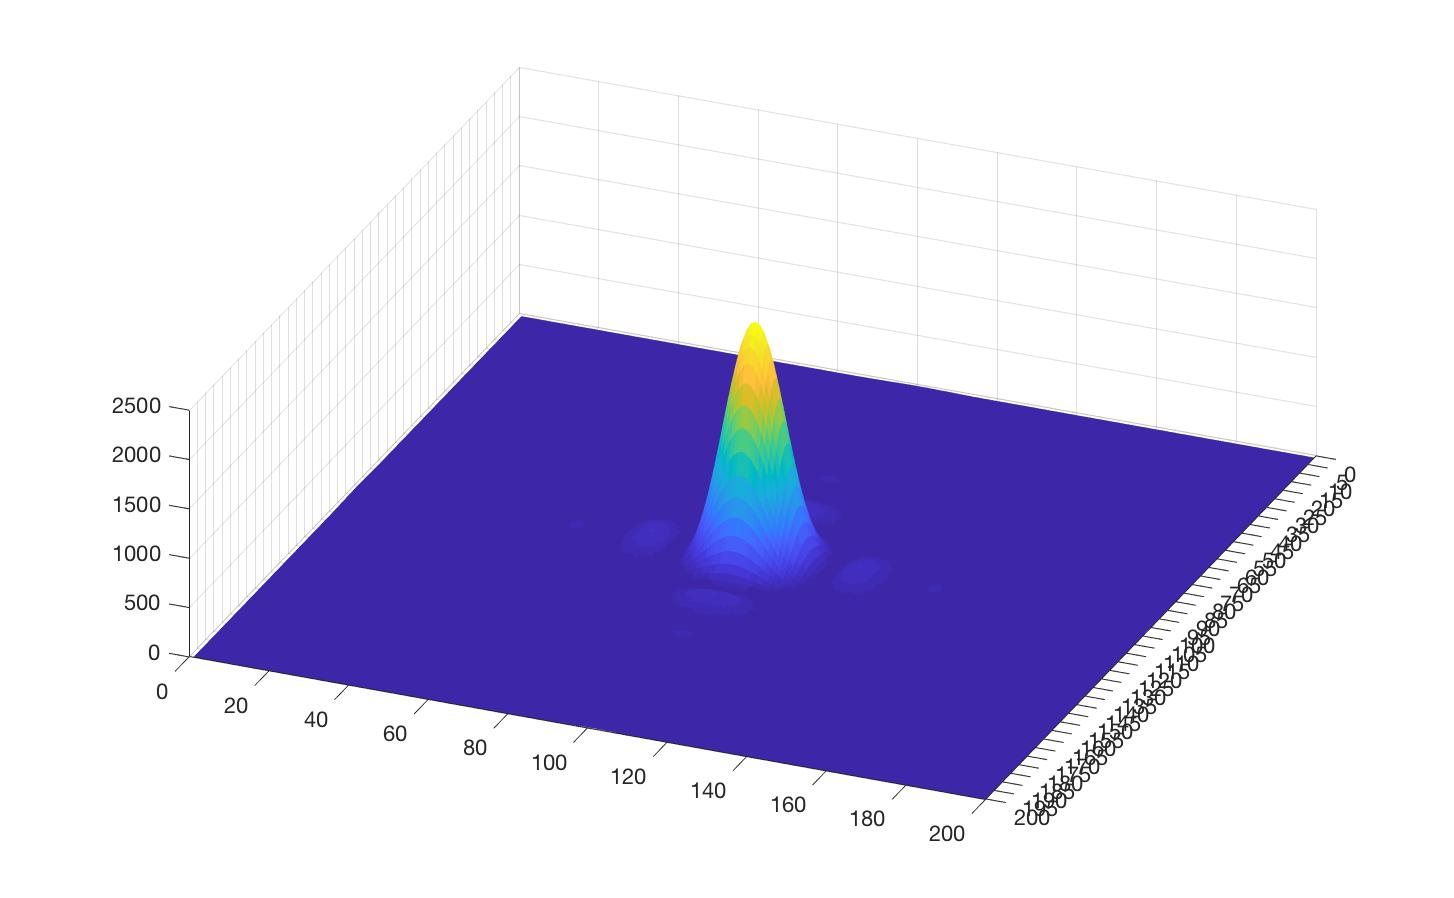
\includegraphics[width=12cm]{figures/Sample.jpg}
    \caption{示例图片}
    \label{fig:sample}
\end{figure}
